\chapter{Vibration Signal Analysis}
\section{Data Collection and Processing}
The most important measurement to be made in order to perform significant rotordynamic analysis is the Vibration Signal, $ V $ or $ W $. Other beneficial measurements include Spin Speed, $ \Omega $, of the rotating shaft (especially important if during a start-up or run-down), and a Reference Signal, $ R $, that indicates a rotational position of the shaft. Orthogonal vibration signals (meaning two independent directions), $ V\ \&\ W $, measuring the position of the shaft centerline can help in characterizing anisotropic systems. Sampling Rates, $ f_s $ of the signals mentioned thus far must be high enough to measure the vibration of interest, typically this is at least several times the highest expected rotation speed of the shaft. It is important to note that these signals can come from an experiment or a theoretical model.\par
There are four variables deduced from the above signals that form the basis for the majority of rotordynamic figures and analysis. These are Amplitude of Vibration, $ A[m,mils] $, Amplitude Spectrum, $ \tilde{A}(\omega)[m,mils] $, Phase of Vibration, $ \beta[\deg,Rad] $, and Spin Speed, $ \Omega[Hz,Rad/s,RPM] $. Amplitude Spectrum is actually a two dimensional variable where the dependent variable, $ \omega[Hz,Rad/s,RPM] $, represents the Frequency of Vibration (or Whirl Speed if its in units of rotation). Figures to be presented in this work are varying combinations of these four variables. The Bode diagram plots $ A $ against $ \Omega $ alongside $ \beta $  against $ \Omega $. A Spectrum figure plots $ \tilde{A}(\omega) $. An extension of this is the Cascade which adds the third dimension of $ \Omega $. Orbit plots represent one cycle of the time domain signals $ V\ \&\ W $. Lastly, 3D Orbits are formed by plotting the orbit($ V,W $) against $ \Omega $. Explanations of the importance and methods in producing these plots are to follow. \par
A difficulty in rotordynamic analysis arises in the continuous change of $ \Omega $ causing a continuous change in the dependent variables $ A,\ \tilde{A}(\omega),\ \&\ \beta $, a visualization of these changes is visualized in Figure \ref{fig:PosOverTime}. This poses difficulty because the techniques used to produce $ A,\ \tilde{A}(\omega),\ \&\ \beta $ from $ V,\ W\&\ R $ rely on a span of subsequent rotations. A solution to this dilemma utilized in this work is the discretization of signals $ X,\ Y,\ R\ \&\ \Omega $ into windows in time. The window, whose width will be represented by the variable $ nspw[samples] $. There is a trade off between accuracy and resolution of variables as $ nspw $ is changed. This trade off will be elaborated on in \S\ref{Resolution}.\par 
\begin{figure}
	\centering
	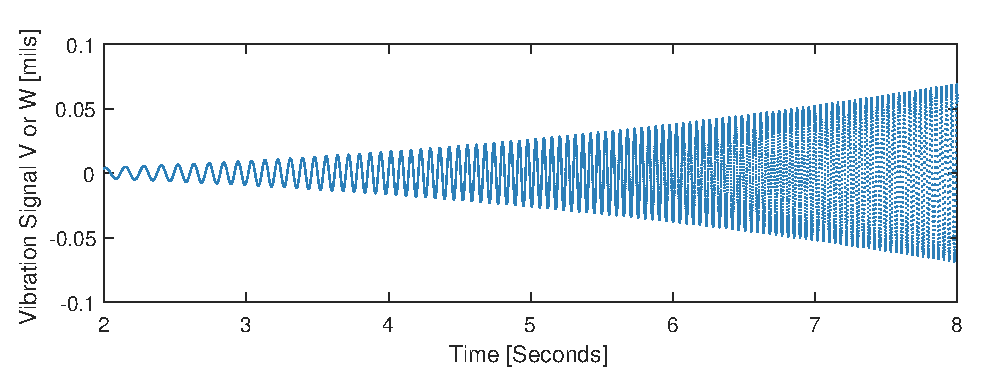
\includegraphics[width=\linewidth]{./figures/Pos_Over_Time.eps}
	\caption{Position of the rotor shaft over a certain timespan.}
	\label{fig:PosOverTime}
\end{figure}
The windowing approach is visually depicted using $ \Omega $ in figure \ref{fig:SpeedWindow} as it changes over time. When the width of the window is small enough, such as in Figure \ref{fig:FreqSpanWindow}, the change in the independent variable becomes vanishingly small. Other continuous variables such as $ A,\ \tilde{A}(\omega),\ \&\ \beta $ are expected to behave similarily, in that their value may be approximated by a single number, or in the case of $ \tilde{A}(\omega) $ as a single spectrum, inside the window despite the change in that variable throughout the entire length of time.
\begin{figure}
	\begin{subfigure}{.5\textwidth}
	\centering
	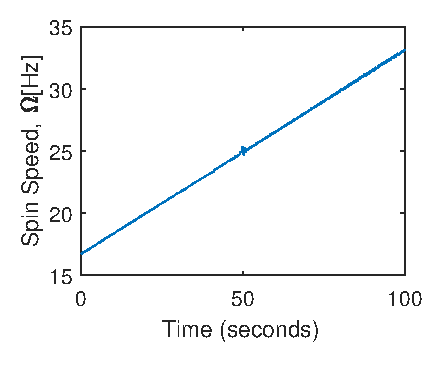
\includegraphics[]{./figures/FrequencySpan.eps}
	\caption{Rotor speed change over time during a ramp up.}
	\label{fig:FreqSpanOverTime}
\end{subfigure}
\begin{subfigure}{.5\textwidth}
	\centering
	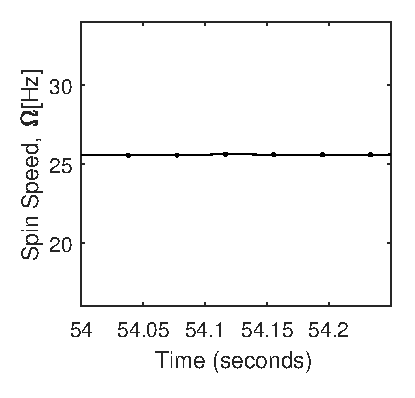
\includegraphics{./figures/FrequencyWindow.eps}
	\caption{Rotor speed change over time during a ramp up.}
	\label{fig:FreqSpanWindow}
\end{subfigure}
\caption{Rotor Spin Speed Windowing effect.}
\label{fig:SpeedWindow}
\end{figure}
Inside of a window of vibration, as the one shown in Figure \ref{fig:WindowedData} the Speed, Amplitude and Phase all approach constant the smaller $ nspw $ gets.\par
\begin{figure}
	\centering
	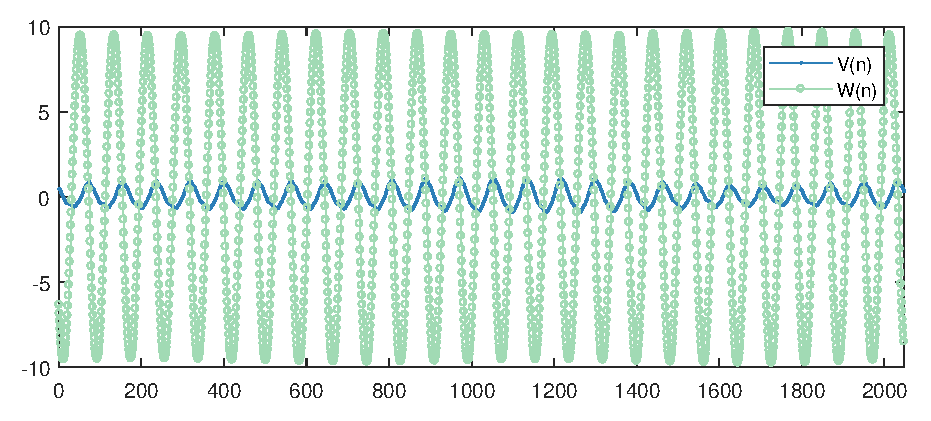
\includegraphics{./figures/SSTime.eps}
	\caption{A window in time of the transient vibration signals for a window, $ nspw $, of $ 2048[samples] $.}
	\label{fig:WindowedData}
\end{figure}
The variables $ V(t) $, $ W(t) $\& $ R(t) $ will now take the form $ V(n) $, $ W(n) $\& $ R(n) $ inside the window (fig. \ref{fig:WindowedData}), where $ n $ is sample number. Spin Speed is simply taken as an average in the window, $ \Omega(N)=avg(\Omega(0:nspw)) $, where $ N $ is the current window index. Therefore, no further explanation is given for its determination. Amplitude, Phase, Amplitude Spectrum, and Spin Speed must be calculated in each window, for a series of windows that cover the entire length of signals. Then a vector of each variable will exist where the length is equal to the number of windows, $ NW $, and is given by
\begin{equation*}
NW = \frac{length(signals)}{nspw}
\end{equation*}\par 
The calculation of each of the variables inside the window, at some $ N $, is given in the following sections. A useful visual representation of the windowed signals $ V(n)\ \& W(n) $ are presented in Figure \ref{fig:WindowedData} to aid in understanding the sections to follow.
\subsection{Amplitude}
Amplitude calculation is fairly straightforward within the window. One approach to calculate the peak to peak amplitude is to take the average over the whole window, $ A_v(N) = max(V(0:nspw))-min(V(0:nspw)) $. Another is to use a peak-finding algorithm to determine the height of each peak and average them all over the sample length. General computer code packages, such as MATLAB,  will contain a peak finding algorithm, the details of which are out of the scope of this work.
\subsection{Spectrum}
The frequency spectrum of the signal is calculated inside the window using a Fourier Transform. In MATLAB the Fast Fourier Transform (fft) has been preprogrammed allowing easy working between time and frequency domains.
\begin{equation}\label{eq:FFTReal}
\tilde{A_V} = \frac{\text{fft}(V)}{nspw},\ \&\ \tilde{A_W} = \frac{\text{fft}(W)}{nspw}
\end{equation}\par 
A useful way to represent the data is using complex variable to compact the two orthogonal displacements $ V\ \&\ W $ as
\begin{equation}\label{eq:ComplexDisplacement}
Z = V + iW
\end{equation}
now the spectrum of this complex value represents both equation planes of vibration in one equation:
\begin{equation}\label{eq:FFTComplex}
\tilde{A}_\pm = \frac{\text{fft}(Z)}{nspw}
\end{equation}\par
Thus far, the frequency spectrum in the real coordinates and in the complex is in terms of samples on the dependent axis. The frequency vector to which the fft() corresponds must be calculated. This is the whirl speed, $ \omega $. It is known that the slope of $ \omega $ is $ d\omega=f_s/nspw $. It is also known that the frequency vector is the same length as the time domain signal 
\begin{equation*}
f(n)=d\omega(0:nspw-1)
\end{equation*}
and to center the spectrum at a frequency of 0
\begin{equation*}
\begin{array}{c}
Q=ceiling((nspw+1)/2)\\
\omega_Q=d\omega(Q-1)\\
\omega=f-fQ
\end{array}
\end{equation*}
where $ \omega $, here in $ Hz $, is the dependent variable that pairs with the real or complex Amplitude spectrum. The Amplitude spectrum in real coordinates(fig.\eqref{eq:FFTReal}) is symmetric for positive and negative $ \omega $, so typically when the spectrum of a single variable is presented in a spectrum plot or in a cascade it is only the positive frequency side presented. On the other hand, the complex representation of the amplitude spectrum(\eqref{eq:FFTComplex}) is not symmetric on the positive and negative sides of $ /omega $. This decomposition can be better understood by realizing the form of the Fourier transform as the summation of circles in the complex plane, $ \tilde{A_\pm}(\omega)e^{i\omega t} $. When $ \omega $ is positive this represents a positive rotation, and when negative represents a negative rotation. For a given whirl speed, $ \omega_i $, this results in sum of a positively rotating circle of amplitude, $ \tilde{A}(\omega_i) $ and a negatively rotating circle of amplitude $ \tilde{A}(-\omega_i) $. The ellipse formed by this summation is the orbit of the shaft centerline at this specific speed. With the understanding of contributions of $ \tilde{A}(\omega) $ and $ \tilde{A}(-\omega) $, we can realize that the resulting ellipse will rotate in the positive direction if $ \tilde{A}(\omega)> \tilde{A}(-\omega) $ and in the negative direction otherwise.
\subsection{Phase}
\subsubsection{Time Domain Approach}
A rather direct way of calculating the phase angle comes from an inspection of the time domain signal. If some once per turn reference is available, then using either a zero-crossing, peak-finding, or threshold algorithm can be employed to reference a specific angle of the shaft rotation. If the vibration signal is mostly synchronous, that is vibrating at the same frequency as the rotation of the shaft, then a peak-finding or zero-crossing algorithm can be used to determine the number of samples from the shaft reference angle to the peak of the vibration.\par 
\begin{equation}\label{eq:PhaseAngleTimeDomain}
\beta_k = 2\pi\frac{\#ref_k-\#peak_k}{\#ref_k-\#ref_{k-1}}
\end{equation}
where $ \beta_k $ is the phase lag of the signal of interest from the reference signal at the $ k $th reference cycle, $ \#ref_k $ is the sample number of the reference trigger, and $ \#peak_i $ is the sample number of the peak of the signal of interest. One large advantage to this brute force method is that is can run continuously and provide current phase information on just the last rotation of the shaft. In the application to the window of vibration data, fig. \ref{fig:WindowedData}, the measurements of each cycle would be averaged across the window as $ \beta(\omega)=avg(\beta_k) $ for however many indexes $ k $ were found in the window. \par 
\subsubsection{Frequency Domain Approach}
Alternatively, the phase angle can be determined using the frequency domain signals.\par 
If the speed of the rotor is known and the time domain signals $ v\ \&\ w $ are known to be synchronous, or filtered to synchronous, then the spectrums of the signals of interest can be used to calculate the phase delay. For any frequency, $ \omega $ the angle is calculated using the equation
\begin{equation*}
\beta(\omega)=angle(\tilde{A}(\omega))-angle(\tilde{K}(\omega))
\end{equation*}
where $ \tilde{K} = \frac{\text{fft}(K)}{nspw} $ is the frequency domain representation of the reference signal. Either $ \tilde{A}_V $ or $ \tilde{A}_W $ is used to find the phase delay of the $ V $ or $ W $ time domain vibration in reference to the once per turn reference of $ K $. It is also possible to find the delay of any time domain signals in reference to any other time domain signal at a specific frequency using the above equation. Though the common practice is to compute the $ \beta $ angle of both signals and subtract one from another. In synchronous vibration, $ \omega=\Omega $.\par
\section{Rotordynamic Figures}\label{ExperimentalPlots}
In the previous section Amplitude, Phase, and frequency spectrum were calculated for the interior of a window of index $ N $. Each of the data then need to be indexed as all of the windows are processed until the entire signal has been exhausted. The total number of windows can be realized in the equation $ NW=\frac{length(X)}{nspw} $ where $ X $ is a placeholder for any time domain signal. After all windows have been exhausted, vectors for $ A,\ \tilde{A}(\omega),\ \beta\ \&\ \Omega $ will all be of length $ NW $.\par 
For the visualization of the plots, experimental data from a overhung rotor system with one disk will used to present the figures.\par
\subsection{Bode}
The Bode diagram for the example overhung rotor system is given in Figure \ref{fig:ExpExampleBode}. First, by looking at the amplitude portion of the plot it si evident that the $ V $ signal undergoes a natural frequency before the $ W $ signal because the peak for $ A_V $ occurs before $ A_W $. This idea is also supported through the inspection of the phase lag portion of the plot, as two seperate transitions are evident. Having two seperate peaks is an indication of high anisotropy of stiffness in the system. By observing the phase lag of each the vertical and the horizontal, it is evident that the orbit direction is opposite the spin speed between speeds ~ 1280-1350[RPM]. This is due to the phase angles switching polarity with one another. If normally horizontal lags vertical, as is suggested by the sub-synchronous and super-synchronous range, then during the critical speed the orbit is reversed since vertical begins to lag horizontal.\par
Bode diagrams are extremely useful in diagnosing unbalance in the system through inspection of the phase lag portion. If the shaft was perfectly straight before any deformation due to rotating unbalance, then the phase lag just before the first natural frequency is the angle of the unbalance vector. This is due to the fact that before the first natural frequency, the unbalance vector is aligned with the vibration radially out from the center of rotation. Furthermore, natural frequencies can be detected through the use of the phase lag information. Phase lag typically shifts $ 180\deg $ through a natural frequency, and is at $ 90\deg $ during one.
\begin{figure}
	\centering
	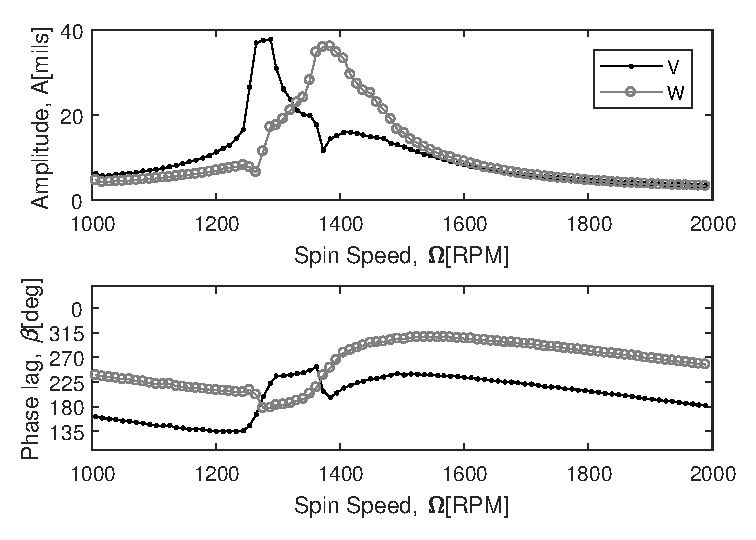
\includegraphics[]{./figures/ExpExampleBode.eps}
	\caption{Bode diagram of the experimental example overhung system. Signals are filtered to synchronous speed.}
	\label{fig:ExpExampleBode}
\end{figure}
\subsection{Full Spectrum and Full Spectrum Cascade}
A single Spectrum at a specific speed is shown as Figure \ref{fig:ExpExampleSpectrum}. This is the Complex representation of the spectrum refered to as the ``Full Spectrum'' of the time domain signal because it contains both positive and negative frequencies. This figure tells us that the orbit at this speed is in the negative whirl direction since the negative amplitude, $ \tilde{A}_\pm(-\omega)=10.27 $ at its peak is greater than $ \tilde{A}_\pm(\omega)=8.80 $. Also, there is minimal amplitude in the spectrum other than this single frequency of $ 31.25[Hz] $ indicating the vibration is highly synchronous.
\begin{figure}
	\centering
	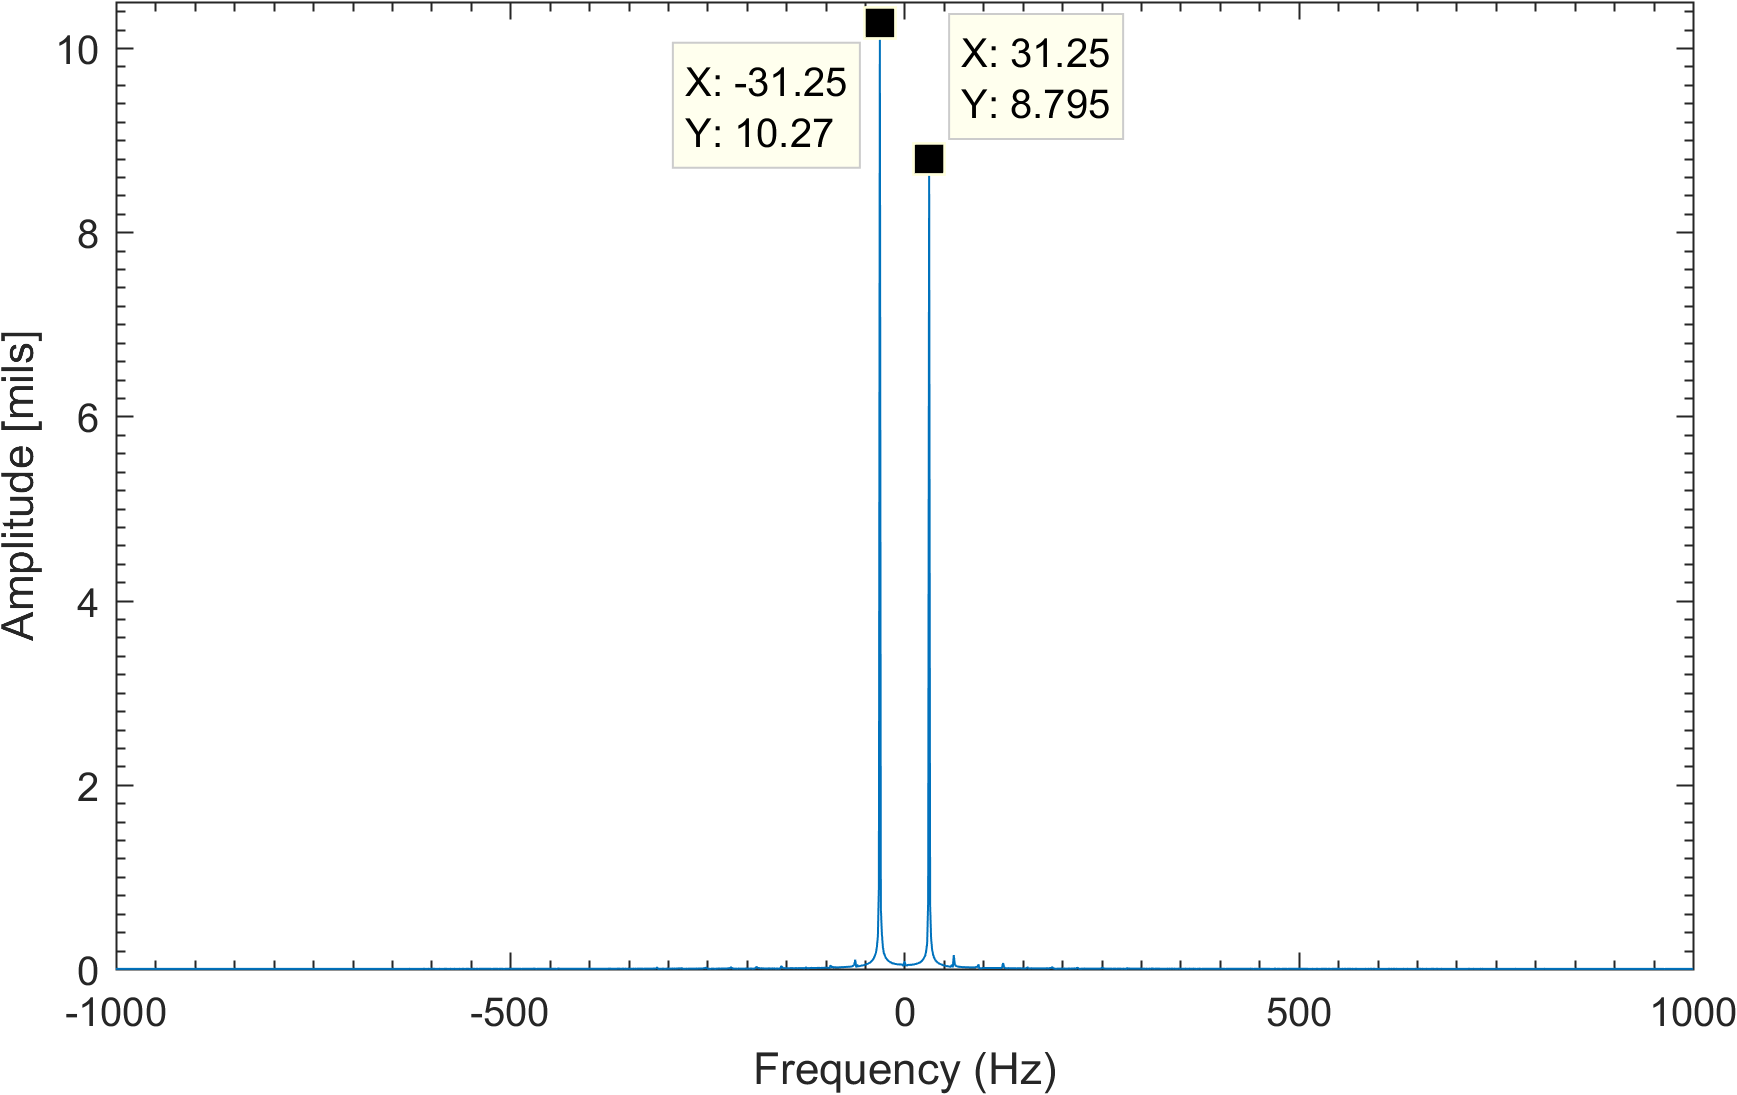
\includegraphics[width=\linewidth]{./figures/Images/Figure_8.png}
	\caption{Example Full Spectrum.}
	\label{fig:ExpExampleSpectrum}
\end{figure}
 A Cascade plot is demonstrated with the experimental system described in \S\ref{ExperimentalPlots}, as Figure \ref{fig:ExpExampleCascade}. Using this figure it is easy to detect the portion of the start-up in which the orbit is whirling opposite the spin speed. A sharp dip in positive amplitude, $ \tilde{A}_\pm(\omega) $, correlated with a sharp rise in negative amplitude, $ \tilde{A}_\pm(-\omega) $, leads to this phenomena.\par 
The Cascade plot is particularly useful in characterizing non-synchronous vibration. Slightly evident in the example cascade of figure \ref{fig:ExpExampleCascade} is the super-synchronous vibration at twice the spin speed, this is often called the 2X vibration and likewise and other non-synchronous whirl can be referenced as nX. The cascade plot is an indispensable tool for the analysis of fluid film bearing as they are characterized by sub-synchronous whirl that is difficult to identify in a Bode Diagram.\par 
\begin{figure}
	\centering
	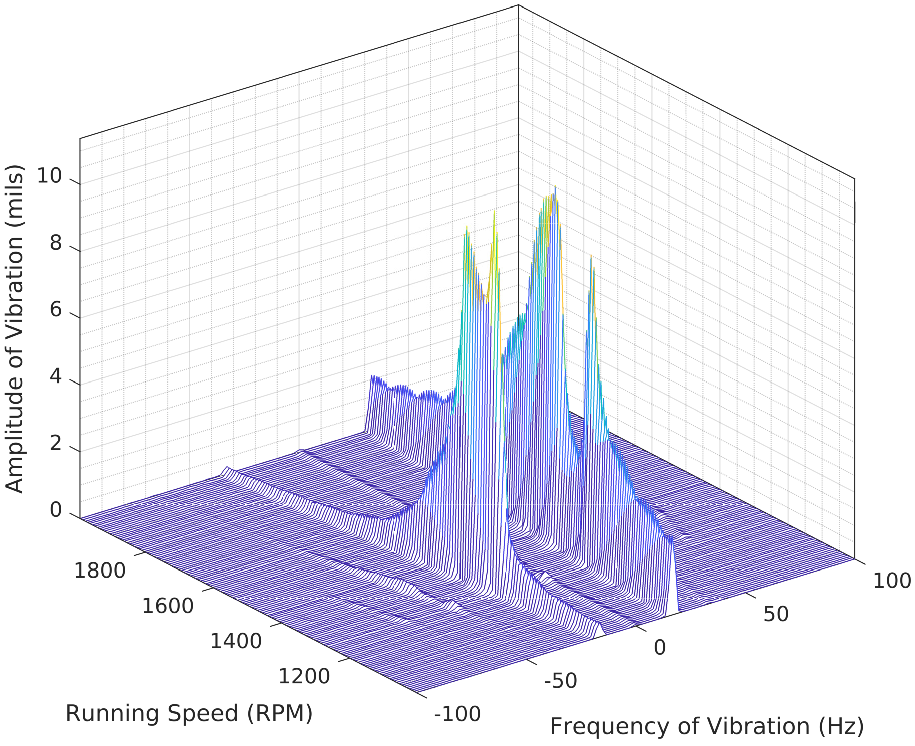
\includegraphics[width=\linewidth]{./figures/ExpExampleCascade.pdf}
	\caption{Cascade of the experimental system described in \S\ref{ExperimentalPlots}.}
	\label{fig:ExpExampleCascade}
\end{figure}
\subsection{Orbit}
Now in the time domain, the actual orbit or trace of the centerline of the shaft is observed. In this work, the orbit is visualized in two ways; as a path in 2D space at a specific spin speed, or as a 3D orbit with a cascade of orbits as spin speed is increased. The 3D Orbit allows for the visualization of complex phenomena in a simple intuitive way. Figure \ref{fig:ExpExample3DOrbit} 3D Orbit is given for the experimental example described in \S\ref{ExperimentalPlots}. Appearing, once again is evidence of the negative whirl in the critical speed range. In the 3D orbit a necking of the shape can be seen between the speeds of 1200-1400[RPM] indicating the orbit has reversed its direction. Looking at independent orbits at specific speeds should explicitly demonstrate the orbit necking and turning negative. In Figure \ref{fig:ExpExampleOrbits} at speed $ 1194[RPM] $ the orbit is clearly whirling in the positive direction, as speed increases the orbit collapses into a line between speeds $ 1203\ \&\ 1206[RPM] $ and begins whirling in the negative direction until the process is reversed by speed $ 1289[RPM] $. Therefore, it can be confirmed that the orbit is whirling backward between the speeds ~1205-~1280[RPM].\par
\begin{figure}
	\centering
	\includegraphics[width=\linewidth]{./figures/ExpExample3DOrbit.eps}
	\caption{3DOrbit of the experimental system described in \S\ref{ExperimentalPlots}. Lighter colors indicate larger vibration.}
	\label{fig:ExpExample3DOrbit}
\end{figure}
\begin{figure}
\begin{subfigure}{.28\linewidth}
	\def\width{\linewidth}
	\pgfplotsset{every picture/.style={scale=1},every axis/.style={title style={yshift=-.8em}}}%, every axis/.style={hide axis}}%
	\centering
	\import{figures/}{ExpExampleOrbit1194.tex}
	\label{fig:ExpExampleOrbit1194}
\end{subfigure}
\begin{subfigure}{.28\linewidth}
	\def\width{\linewidth}
	\pgfplotsset{every picture/.style={scale=1},every axis/.style={title style={yshift=-.8em}}}%, every axis/.style={hide axis}}%
	\centering
	\import{figures/}{ExpExampleOrbit1203.tex}
	\label{fig:ExpExampleOrbit1203}
\end{subfigure}\vspace{-2em}
\begin{subfigure}{.28\linewidth}
	\def\width{\linewidth}
	\pgfplotsset{every picture/.style={scale=1},every axis/.style={title style={yshift=-.8em}}}%, every axis/.style={hide axis}}%
	\centering
	\import{figures/}{ExpExampleOrbit1206.tex}
	\label{fig:ExpExampleOrbit1206}
\end{subfigure}
\begin{subfigure}{.5\linewidth}
	\def\width{.55\linewidth}
	\pgfplotsset{every picture/.style={scale=1},every axis/.style={title style={yshift=-.8em}}}%, every axis/.style={hide axis}}%
	\centering
	\import{figures/}{ExpExampleOrbit1222.tex}
	\label{fig:ExpExampleOrbit1222}
\end{subfigure}
\begin{subfigure}{.5\linewidth}
	\def\width{.55\linewidth}
	\pgfplotsset{every picture/.style={scale=1},every axis/.style={title style={yshift=-.8em}}}%, every axis/.style={hide axis}}%
	\centering
	\import{figures/}{ExpExampleOrbit1289.tex}
	\label{fig:ExpExampleOrbit1289}
\end{subfigure}
\caption{Orbits of the experimental example. Spin speed is counterclockwise. Blue dots indicate the reference position of the shaft, and the beginning of each orbit.}
\label{fig:ExpExampleOrbits}
\end{figure}

\subsection{Filtering}
Correlating phase angles between real signals can be extremely difficult due to the noise and harmonic frequencies that may disrupt the measurement. Furthermore, it can be useful to decompose a real signal into specific harmonic components of the spin speed. One such instance is in the analysis of a fluid film bearing. Often the fluid film bearing will cause an unbalance at the subsynchronous frequency of just under 0.5X. Using a filter, the response of the system to this specific frequency can be extracted, allowing the analysis of phase angle and amplitude directly due to the influence of interest.\par 
MATLAB has an extensive library of digital filters that can be adjusted to filter specific frequency ranges with no phase delay, and recall the states from the previous window as to not loose dynamic information from one step to the next.\par 
A synchronous filter was applied the experimental example and the cascade plot is shown in Figure \ref{fig:ExpExampleCascade2}. All amplitudes of frequencies other than the synchronous frequencies have been eliminated. This system did not have strong super- or sub-synchronous response, so this filtering does not make an appreciable effect to the Bode plot. But, with many real systems filtering will be necessary to analyze the system.
\begin{figure}
	\centering
	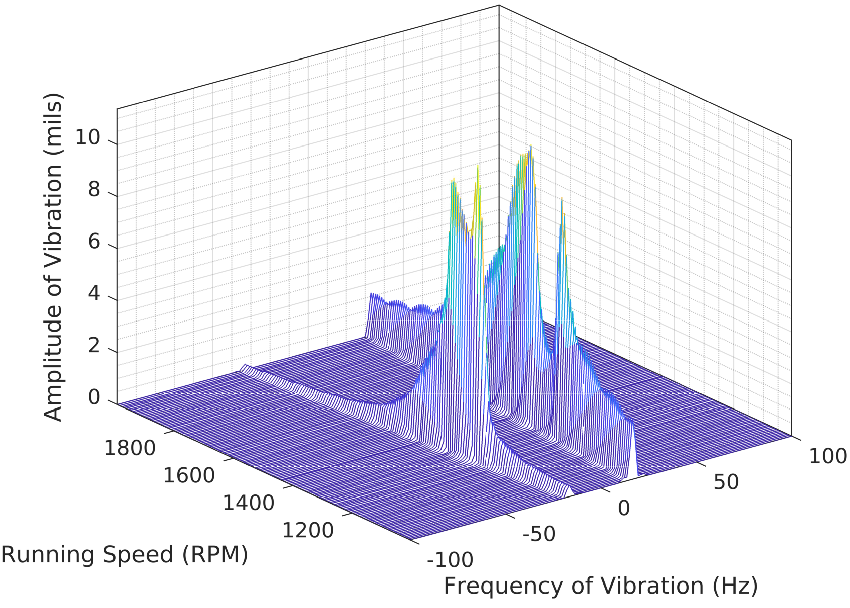
\includegraphics[width=\linewidth]{./figures/ExpExampleCascade2.pdf}
	\caption{Cascade of the experimental system witha synchronous filter applied.}
	\label{fig:ExpExampleCascade2}
\end{figure}